
\begin{figure}
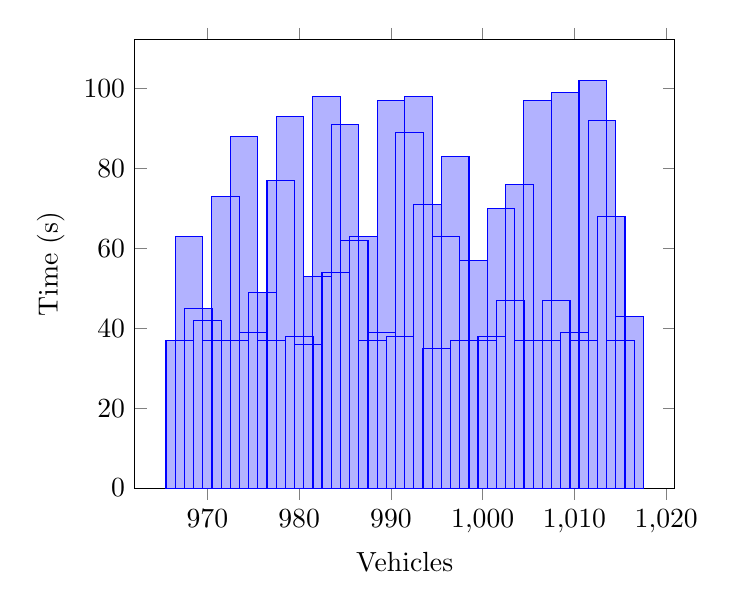
\begin{tikzpicture}
\begin{axis}[
legend style={anchor=west},
xlabel=Vehicles,
ylabel=Time (s),
ymin=0,
ybar,
]
\addplot coordinates {
(1005, 37)
(1014, 68)
(1015, 37)
(1016, 43)
(1010, 39)
(1011, 37)
(994, 71)
(1013, 92)
(1002, 70)
(1006, 97)
(972, 73)
(1009, 99)
(1008, 47)
(1007, 37)
(1004, 76)
(1000, 37)
(977, 37)
(976, 49)
(975, 39)
(974, 88)
(973, 37)
(971, 37)
(970, 42)
(979, 93)
(978, 77)
(1012, 102)
(995, 35)
(997, 83)
(996, 63)
(991, 38)
(990, 97)
(993, 98)
(992, 89)
(999, 57)
(998, 37)
(1003, 47)
(967, 37)
(968, 63)
(969, 45)
(988, 37)
(989, 39)
(982, 53)
(983, 98)
(980, 38)
(981, 36)
(986, 62)
(987, 63)
(984, 54)
(985, 91)
(1001, 38)
};

\end{axis}
\end{tikzpicture}
\label{tik:time:0:90}
\caption{0 percent diving with GSC on route $90$}
\end{figure}
